\chapter{Adversarially Learned Transformations for Single-Source Domain Generalization}
\label{chap:alt}
In Chapter~\ref{chap:agat}, we looked at a relaxed setting of the generalization problem -- in that setting, information about the target domain was available in terms of a set of attributes that are known to differ at test time.
% (target samples are not available).
In this chapter we will go beyond attributes and address the harder and broader problem of domain generalization.

% As discussed earlier, domain generalization is the problem of making accurate predictions on previously unseen domains, especially when these domains are very different from the data distribution on which the model was trained. 
% In this chapter, we will tackle an even harder problem -- \textit{single source domain generalization (SSDG)}, where the model has access only to a single training domain, and is expected to generalize to multiple different testing domains. 
% This is especially hard because of the limited information available to train the model with just a single source. 

% \section{Introduction}
\begin{figure}
    \centering
    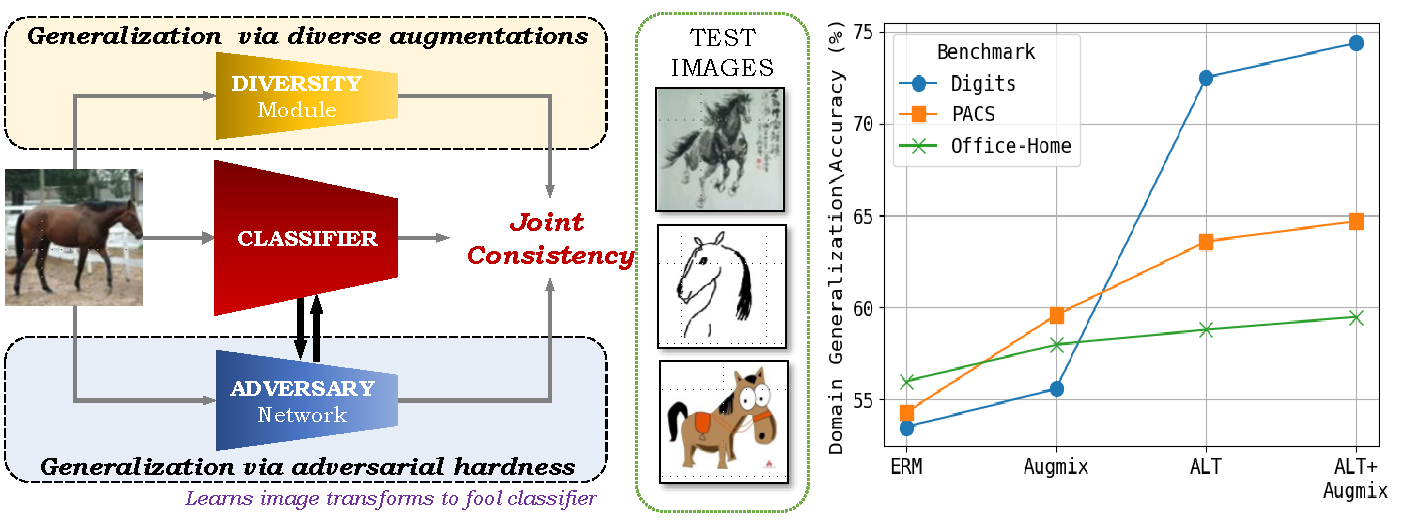
\includegraphics[width=\linewidth]{alt/figures/alt_teaser.pdf}
    \caption{
    This figure illustrates our approach which consists of a \textit{diversity} module (data augmentation functions such as Augmix~\citep{hendrycks2019augmix} or RandConv~\citep{xu2020robust}) and an \textit{adversary} network (ALT) (to learn image transformations that fool the classifier).
    We show an example from the PACS benchmark under the single-source domain generalization setting, with real photos (P) as the source domain and art paintings (A), cartoons (C), and sketches (S) as the target domains.
    The plot summarizes our results -- while diversity alone improves performance over the naive ERM baseline, adapting this diversity using adversarially learned transformations (ALT) provides a significant boost for domain generalization on multiple benchmarks.}
    \label{fig:alt_teaser}
\end{figure}


Domain generalization is the problem of making accurate predictions on previously unseen domains, especially when these domains are very different from the data distribution on which the model was trained. 
This is a challenging problem that has seen steady progress over the last few years \citep{carlucci2019domain,volpi2018generalizing,qiao2020learning,xu2020robust,nam2021reducing}. 
this chapter focuses on the special case -- single source domain generalization (SSDG) -- where the model has access only to a single training domain, and is expected to generalize to multiple different testing domains. 
This is especially hard because of the limited information available to train the model with just a single source. 

In the case where multiple training domains (i.e., multi-source DG) are available, recent analysis \citep{gulrajani2021in} shows that even simple methods like minimizing empirical risk jointly on all domains, performs better than most existing sophisticated formulations.
% on par with sophisticated formulations.
A corollary to this finding is that success in 
%SSDG
domain generalization is primarily dependent on \emph{diversity} -- i.e., exposing the model to as many potential training domains as possible.
As the SSDG problem allows access only to a single training domain, such an exposure must come in the form of diverse transformations of the source domain that can simulate the presence of multiple diverse domains ultimately leading to low generalization error. 
% which in this case must be in the form of diverse transformations of the source domain that can simulate the presence of multiple different domains ultimately leading to low generalization error. 

The idea of using diversity to train better models has been sufficiently explored -- many recent approaches have shown that a diverse set of augmentations during training improves a model's robustness under distribution shifts \citep{hendrycks2019augmix,yun2019cutmix,zhang2018mixup,cubuk2020randaugment}. 
However, the extent to which the model needs to be exposed to the diverse transformations is unclear, and over-exposure may hurt the model's generalization capabilities. 
Moreover, these methods define a strong prior in terms of the types of diversity that is desirable -- for e.g., in object recognition tasks, invariance to affine transformations, color jitter, blurs, or other kinds of pixel noise is desirable. 
Specific augmentations can be used if the type of diversity encountered at test time is known; for instance if it is known that the test set may contain random combinations of rotation, translation, and scaling, using augmentations that are correlated with this domain shift would lead good performance~\citep{gokhale2021attribute,benton2020learning,wong2020learning}.

Unfortunately, by design, these methods can only achieve invariance under small distribution shifts, like unknown corruptions, noise or imperceptible and perceptible adversarial attacks. 
These methods typically do not work effectively when the distribution shift is large and of a semantic nature, as in the case of domain generalization. 
On the other hand, some recent methods have directly used randomized convolutions to synthesize diverse image manipulations~\citep{xu2020robust}, motivated by the large space of potentially realizable functions induced by a convolutional layer, which cannot be easily emulated using simple analytical functions. 
 
In this chapter we hypothesize that, while diversity is critical in order to succeed in single domain generalization, diversity alone is insufficient. 
In other words, blindly exposing a model to a wide range of transformations cannot improve the generalization performance. Instead, we argue that other carefully designed forms of diversity are needed -- specifically those that can expose the model to unique, and task-dependent transformations with large semantic changes that are otherwise unrealizable with plug-and-play augmentations as before.  To this end, we introduce an adversary network whose objective is to find plausible image transformations that maximize classification error. We enforce a consistency between a \textbf{diversity module} and the \textbf{adversary network} during training along with the classifier's predictions. 

Our method, dubbed ALT (adversarially learned transformations), offers an interplay between diversity and adversity. Over time, a synergistic partnership between the diversity and adversary networks emerges, exposing the model to increasingly unique, challenging and semantically diverse examples that are ideally suited for single source domain generalization.  The adversary network benefits from the classifier being exposed to the diversity module, and as such avoid trivial adversarial samples with appropriate checks. This allows the adversarial maximization to explore a wider space of adversarial transformations that cannot be covered by prior work on pixel-level additive perturbations.
  
We demonstrate this advantage of our method empirically on multiple benchmarks -- PACS \citep{li2017deeper}, Office-Home \citep{venkateswara2017deep}, and Digits \citep{volpi2018generalizing}. On each benchmark, we outperform the state-of-the-art single source domain generalization methods by a significant margin.  Moreover, since our framework disentangles diversity and adversarial modules, we can combine it with various diversity enforcing techniques -- we identify two such state-of-the-art methods with AugMix \citep{hendrycks2019augmix}, and RandConv \citep{xu2020robust}, and show that placing them inside our framework leads to significantly improved generalization performance over their vanilla counterparts. 
We illustrate this idea in figure \ref{fig:alt_teaser} where we show an image of a horse from the 'photo' training distribution in PACS and the different styles of cartoon/sketch/art painting horses that may be encountered at test time. 

\paragraph{Contributions:}
We summarize our contributions below:
\begin{itemize}[nosep,noitemsep,leftmargin=*]
    \item We introduce a method, dubbed ALT, which produces adversarially learned image transformations that expose a classifier to a large space of image transformations for superior domain generalization performance. ALT performs adversarial training in the parameter space of an adversary network as opposed to pixel-level adversarial training.
    \item We show how ALT integrates diversity-inducing data augmentation and hardness-inducing adversarial training in a synergistic pipeline, leading to diverse transformations that cannot be realized by blind augmentation strategies or adversarial training methods on their own.
    \item We validate our methods empirically on three benchmarks demonstrating state-of-the-art performance, and provide insights into and analysis of approach.
\end{itemize}

% Instead, the model must be able to trade-off diversity and classifier performance as needed such that it achieves 'optimal' exposure in a given task, and no more --  which is challenging to define \emph{a priori}. Instead, we are able to achieve this trade-off using a consistency using an additional network that acts an adversary to the classifier by learning adversarial transformations of the input image for every single batch during training. By randomly initializing this network in each iteration, we ensure the adversarial transformations are unique, and diverse themselves. We then place a consistency objective between the diverse and adversarial transformations so together they expose the model to learn from both diverse and challenging domains
% \section{Related Work}
\textbf{Domain Generalization}
has been explored under both multi-source (MSDG) and single-source (SSDG) settings. Techniques designed for MSDG seek to utilize the multiple domains to perform feature fusion~\citep{shen2019situational}, learning domain-invariant features~\citep{ganin2016domain}, meta-learning~\citep{li2018learning}, invariant risk minimization~\citep{arjovsky2019invariant}, learning mappings between multiple training domains~\citep{robey2021model}, and style randomization~\citep{nam2021reducing}.
Gulrajani  \textit{et al.}~\citep{gulrajani2021in} provide an extensive comparative study of these approaches and report that simply performing ERM on the combination of source domains leads to the best performance. Many benchmarks have been proposed to evaluate MSDG performance such as PACS~\citep{li2017deeper}, OfficeHome~\citep{venkateswara2017deep}, Digits~\citep{volpi2018generalizing}, and WILDS~\citep{koh2021wilds} which is a compendium of MSDG datasets for various tasks such as image classification, text sentiment classification, text toxicity prediction, etc. In the context of multi-source DG, \citep{zhou2020learning} propose to synthesize novel domains using a conditional generator trained on multiple domains using cycle consistency -- whereas we are primarily interested in the single source setting where such a method may not be feasible. Moreover, we strictly synthesize novel domains as functions of the source domain, and place emphasis on the nature of functions that are learnable during training with a convolutional network with objectives such as an adversarial cost and consistency measures.

SSDG is a harder setting due to the lack of multiple datasets for using the above methods; most work in SSDG has therefore focused on data augmentation.
Notable among these methods is the idea of adversarial data augmentation -- ADA\citep{volpi2018generalizing} and M-ADA~\citep{qiao2020learning} apply pixel-level additive perturbations to the image in order to fool the classifier.  Resulting images are used as augmented data to train the classifier.
% is trained over the union of source dataset and adversarial samples.
RandConv~\citep{xu2020robust} shows that shape-preserving transformations in the form of random convolutions of images lead to impressive performance gains on Digits.
% benchmark.

\textbf{Robustness to Image Corruptions.}
There has also been interest in training classifiers that are robust to corruptions that occur in the real world, such as different types of noise and blur, artifacts due to compression techniques, and weather-related environments such as fog, rain, and snow.
\citep{vasiljevic2016examining,geirhos2018generalisation} show that training models with particular types of corruption augmentations does not guarantee robustness to other unseen types of corruptions or even different severities of corruptions. 
Hendrycks~ \textit{et al.}~\citep{hendrycks2018benchmarking} curate benchmarks (ImageNet-C and CIFAR-C) to test robustness along a fixed set of corruptions.
They also provide a benchmark called ImageNet-P which tests robustness against other corruption types such as small tilts and changes in brightness.
A similar benchmark for corruptions of handwritten digit images, MNIST-C~\citep{mu2019mnist} has also been introduced.

% \paragraph{Robustness to Adversarial Attacks}

\textbf{Data Augmentation}
has been an effective strategy for improving in-domain generalization using simple techniques such as random horizontal flips and cropping~\citep{he2016deep}, random occlusion or removal of patches~\citep{devries2017improved,zhong2020random}.
Data augmentation techniques have been shown to improve robustness against adversarial attacks and natural image corruptions~\citep{zhang2018mixup,yun2019cutmix,cubuk2020randaugment}.
Learning to augment data has been explored in the context of object detection~\citep{zoph2020learning} and image classification~\citep{ratner2017learning,cubuk2019autoaugment,zhang2019adversarial}. 
% - previous methods for SSDG: naive data aug, 

% - style changes, style normalization 

% - diversity: augmix, randconv, older random projection papers, 

% - adversarial data aug --- talk about how adv training can only provide resiliency to small perturbations 

%  - newer methods when some info is known about target (but no dataset available) -- agat, perturbation sets rts

\section{Proposed Approach} 
% \paragraph{Preliminaries.}
Under the single-source domain generalization setting, consider the training dataset $\mathcal{D}$ containing $N$ image-label pairs $\mathcal{D} = \{(\xx_i, \yy_i)\}_{i=1}^{N}$, and a classifier $f$ parameterized by neural network weights $\theta$. 
The standard expected risk minimization (ERM) approach seeks to learn $\theta$ by minimizing the the in-domain risk measured by a suitable loss function such as the binary cross-entropy loss.
\begin{equation}
    \mathcal{R}_{ERM} = \underset{\xx\in\mathcal{D}}{\E} \mathcal{L}_{BCE}(f(\xx;\theta), \yy).
    \label{alt:eq:erm}
\end{equation}
For SSDG, we are interested in a classifier that has the least risk on any \textit{unseen} target domain $\mathcal{D}^\prime$ that is not observed during training. Note that in SSDG, there is only domain shift and no label shift, i.e. we assume the same classes exist in the training and testing domains. 
Our approach builds on diversity based and adversarial augmentation approaches which we outline next. 

\paragraph{Generalization via Diversity.} A successful strategy to improve generalization error on unseen domains is to utilize a diverse set of pre-defined transformations, $\mathcal{F}_{div}$, to synthesize data augmentations that emphasize the invariance properties that are important for $f(\theta)$ to learn. Methods that fall under this category modify Equation \ref{alt:eq:erm} as follows: 
\begin{equation}
    \label{alt:eq:div_erm}
    \mathcal{R}_{div} = \underset{\xx\in\mathcal{D}}{\E} \mathcal{L}_{BCE}(f(\xx; \theta), \yy) + \lambda_{KL} D_{KL},
\end{equation}
where $D_{KL}$ is a consistency term, typically a divergence, such as KL-Divergence, between the softmax probabilities of the classifier obtained with the clean and transformed data, respectively, \textit{e.g.}, $D_{KL} = KL(f(\xx) ||f(\mathcal{F}_{div}(\xx)))$. 
When $\mathcal{F}_{div}$ is chosen as a set of pre-defined transformations like shear, rotate, color jitter etc., this approach is referred to as AugMix \citep{hendrycks2019augmix}, and when it is a set of randomly initialized convolutional layers this method becomes RandConv \citep{xu2020robust} -- both of which are among the most effective strategies to enforce diversity-based consistencies for generalization.
Although these methods have the advantage of being simple pre-defined transformations that are dataset agnostic, they suffer from drawbacks under the SSDG setting.
When executed on their own, they may not capture sufficient diversity in terms of \textbf{large} semantic shifts, such as when expecting generalization on sketches from a model trained on photos.
% However, these methods suffer from a few drawbacks -- they are pre-defined and capture a large class of potential image transformations (particularly rand-conv), but when executed on their own, they may not capture sufficient diversity in terms of \emph{large} semantic shifts. 

\paragraph{Generalization via adversarial hardness.}
An alternative approach to domain generalization is via adversarial augmentation  which exposes a classifier to `hard' samples during training -- defined broadly as examples that are carefully designed to cause the model to fail. Such samples are augmented to the training set, with the expectation that exposure to such adversarial examples can improve the model's generalization performance on unseen domains \citep{volpi2018generalizing,qiao2020learning}. This is commonly enforced by learning an additive noise vector which when added, maximizes classifier cost. Unfortunately in the case of domain generalization, these methods have failed to match the performance of diversity-only methods optimizing for the cost outlined in Equation~\ref{alt:eq:div_erm}. This is in part because they lack sufficient diversity, and by design they can only guarantee robustness to small perturbations from the training domain, as opposed to large semantic shifts, which are crucial for domain generalization.

% \begin{equation}
%     \label{alt:eq:div_erm}
%     \mathcal{R}_{adv} = \underset{||\delta||_p < \epsilon}{\textrm{max}}~\mathcal{L}_{BCE}(f(\xx+\delta;\phi); \theta), \yy)
% \end{equation}

\begin{algorithm}[t]
    \caption{Adaptive Diversity via ALT}
    \begin{algorithmic}[0]
        \State \textbf{Input:} Source dataset $\mathcal{D}=\{(\xx_i,\yy_i)\}_{i=1}^N$ 
        \State \textbf{Output:} Learned weights $\theta^*$  
    \end{algorithmic}
    \begin{algorithmic}[1]
        \State \textbf{Initialize:} $\theta\gets\theta_0$ \algorithmiccomment{weights of $f()$}
        \ForEach{$t \in \{1\dots T\}$}%
            \State $\xx_t, \yy_t \sim\mathcal{D}$ \algorithmiccomment{\textit{sample input batch}}
            % \Statex ~~\quad$\triangleright$~\textit{train on source only}
            \If{$t < T_{pre}$} 
                \State $\theta\gets\theta - \eta\nabla \mathcal{L}_{cls}(f(\xx_t;\theta), \yy_t))$ 
            % \Statex ~~\quad$\triangleright$~\textit{ALT}
            \Else
                \State $\rho\gets\rho_0,~\phi\gets\phi_0$\algorithmiccomment{weights of $r()$, $g()$}
                \ForEach{$i\in{1\dots m_{adv}}$}
                    % \State $\phi\sim KN()$ \algorithmiccomment{initialize $\phi$}
                    % \State $\hat{\yy}\gets f(\xx; \theta)$
                    % \State $\xx_g \gets g(\xx;\phi)$
                    \State $\hat{\yy_g} \gets f(g(\xx;\phi);\theta)$
                    % \State $L_{adv} \gets \mathcal{L}_{cls}(\hat{\yy_g}, \yy) - \mathcal{L}_{TV}(\xx_g)$
                    % \State $\phi\gets\phi+\nabla\mathcal{L}_{adv}$
                    \State $\phi\gets\phi+\nabla(\mathcal{L}_{cls}(\hat{\yy_g}, \yy) - \mathcal{L}_{TV}(\xx_g))$
                \EndForEach
                % \Statex ~~\quad~~\quad $\triangleright$ \textit{Consistency}
                % \State $p_c,~p_r,~p_g \gets f(\xx; \theta),~f(r(\xx); \theta),~f(g(\xx); \theta)$
                % \State $p_{mix}\gets (p_c + w_r p_r + (2-w_r)p_g)/3$
                % \State $\mathcal{L}_{KL}\gets\sum_{j\in\{c,r,g\}}D_{KL}(p_{mix}||p_j)$ 
                % \State $\theta\gets\theta-\eta_{adv}\nabla((1-\lambda_{KL})\mathcal{L}_{cls} + \lambda_{KL}\mathcal{L}_{KL})$
                \State $\theta\gets\theta-\eta_{adv}\nabla\mathcal{L}_{ALT}$ \algorithmiccomment{see Eq.\ref{alt:eq:L_KL},\ref{alt:eq:L_ALT}}
            \EndIf 
        \EndForEach
        \State\Return $\theta$
\end{algorithmic}
\label{algo}
\end{algorithm}



\paragraph{Adversarially Learned Transformations (ALT).}
While diversity-only methods have shown promise, they are limited in their ability to generalize to domains with large semantic shifts; on the  other hand, techniques based purely on adversarial hardness are theoretically well-motivated but do not match the performance of diversity-based methods. Instead, in this chapter, we propose a new approach that takes the best of these two approaches using an adversary network that is trained to create \emph{plausible} image transformations that fool the classifier. These manipulated images are then used during training as examples on which the image must learn invariance. Since these perturbations are parameterized as learnable weights of a neural network, the network is free to choose large, complex transformations without being restricted to additive noise as done in previous work~\citep{volpi2018generalizing}. Further, this network is randomly initialized for each batch, making the types of adversarial transformations discovered unique and diverse over the course of training.  
%
% With this goal in mind, we propose learning transformations of source images using an adversarially trained image-to-image transformation network 

Formally, the adversary network transforms the input image as $g\colon\R^{C\times H\times W}\rightarrow\R^{C\times H\times W}$, where $C$, $H$, $W$ are the number of channels, height, and width of input images.
$g$ is parameterized by a set of weights denoted by $\phi$. This network, dubbed ALT, forms the backbone of our method.  To train ALT, we setup an adversarial optimization problem with the goal of producing transformations, which when applied to the source domain, can fool the classifier $f$.
While existing efforts dealing with robustness to small corruptions use pixel-level and $\ell_p$ norm-bounded perturbations to fool the model, we find that this is not sufficient for domain generalization as such methods do not allow searching for adversarial samples with semantic changes.
Instead, we directly perform adversarial training in the space of $\phi$, i.e., the neural network weights of ALT. Given input images $\xx$, parameters $\phi$ are randomly initialized, and the corresponding adversarial samples $\xx_g$ are found as:
\begin{equation}
    \xx_g = \underset{\phi}{\textrm{max}}~\mathcal{L}_{BCE}(f(g(\xx;\phi); \theta), \yy) - \mathcal{L}_{TV}(g(\xx;\phi)). 
    \label{alt:eq:adv_max}
\end{equation}
The first term seeks to update $\phi$ so as to maximizes the classifier loss, while $\mathcal{L}_{TV}$ (total variation)~\citep{rudin1992nonlinear} acts as a smoothness regularization for the generated image $\xx_g = g(\xx;\phi)$. The maximization in Equation \ref{alt:eq:adv_max} is solved by performing $m_{adv}$ steps of gradient descent with learning rate $\eta_{adv}$. We note a few important aspects of ALT -- unlike existing methods that explicitly place an $\ell_p-$norm constraint on the adversarial perturbations, we control the strength of the adversarial examples by limiting the number of optimization steps taken by $g$ to maximize classification error. Next, since we randomly initialize $g$ for each batch, the network is reset to a random function. In fact, when the number of adversarial steps is set to 0, $g$ behaves similar to RandConv \citep{xu2020robust} since its only a set of convolutional layers, with additional non-linearity. Finally, in addition to limiting the number of adversarial steps, we place a simple total variation loss on the generated image to force smoothness in the output. This naturally suppresses high frequency noise-like artifacts and encourages realistic image transformations and prevents the network from learning trivial transformations  -- for e.g., only noise or removing semantic content entirely. 

\paragraph{Improving Diversity.}
The samples $\xx_g$ obtained by solving Equation~\ref{alt:eq:adv_max} represent hard adversarial images that can be leveraged by the model to generalize to domain shift. But it also lends itself to exploit other forms of na\"ive diversity achieved by methods like RandConv and AugMix.
% On the other hand, augmentations such as RandConv and Augmix produce images that represent predefined image transformations such as random scaling, cropping, affine transformations, color jitter and so on.
We represent these ``diversity modules'' as $r$, which produce outputs $\xx_r{=}r(\xx)$. Our method utilizes these samples in the training process by enforcing a consistency between the predictions of the classifier on the source image and its transformations from $r$ and $g$. By including the diversity module into the optimization process, the invariances inferred by the classifier lead to stronger and more diverse adversarial examples in future epochs. 
Eventually, a synergistic partnership emerges between the diversity module and the adversary network to produce a wide range of image transformations that are significantly different from the source domain.  

Let $p_c$, $p_r$, and $p_g$ denote the softmax prediction probabilities of classifier $f$ on $\xx$, $\xx_r$, and $\xx_g$, respectively. Then the consistency between these predictions can be computed using Kullback-Leibler divergence~\citep{kullback1951information} as:
\begin{equation}
    \mathcal{L}_{KL} = D_{KL}(p_{mix}||p_c) + w_r D_{KL}(p_{mix}||p_r) + (2-w_r) D_{KL}(p_{mix}||p_g), 
    \label{alt:eq:L_KL}
\end{equation}
% \begin{equation}
%     \mathcal{L}_{KL} = D_{KL}(p_{mix}||p_c) + w_r D_{KL}(p_{mix}||p_r) 
%     % \nonumber\\
%     + (2-w_r) D_{KL}(p_{mix}||p_g), 
%     \label{alt:eq:L_KL}
% \end{equation}
where $p_{mix}$ denotes the mixed prediction:
\begin{equation}
    p_{mix} = \frac{p_c + w_r p_r + (2-w_r)p_g}{3}.
    \label{alt:eq:p_mix}
\end{equation}
The weight $w_r\in[0,2]$ controls the relative contribution of diversity and adversity to the consistency loss; $w_r>1$ implies that consistency with the diversity module has more weight and $w_r<1$ implies that consistency with the adversary network has more weight.
In all our benchmark experiments, we use $w_r=1$, i.e., both diversity and adversary are given equal importance.

Our final loss function for training the classifier is given as the convex combination of classifier loss $\mathcal{L}_{cls}$ with the consistency $\mathcal{L}_{KL}$:
\begin{align}
    \mathcal{L}_{cls} &= \mathcal{L}_{BCE}(f(g(\xx); \theta), \yy), \label{alt:eq:L_cls}\\
    \mathcal{L}_{ALT} &= (1-\lambda_{KL})\mathcal{L}_{cls} + \lambda_{KL}\mathcal{L}_{KL}.
    \label{alt:eq:L_ALT}
\end{align}


\paragraph{Implementation.}
In practice, ALT is implemented using the pseudocode shown in Algorithm~\ref{algo}.
In our experiments, we use RandConv or AugMix as the diversity module $r$ and a fully-convolutional image-to-image network as the adversary network $g$.
$g$ has 5 convolutional layers with kernel size $3$ and LeakyReLU activation.
We train the classifier for a total of $T$ batch iterations of which $T_{pre}$ iterations are used for pre-training the classifier using standard ERM on only the source domain (with only $\mathcal{L}_{cls}$).
For iterations $t>T_{pre}$, for each batch, we randomly initialize the weights of both $r$ and $g$ with the ``Kaiming Normal'' strategy~\citep{he2016deep} as our starting point for producing diverse perturbations, and update $g$ using the adversarial cost in Equation~\eqref{alt:eq:adv_max}.
After $g$ is adversarially updated for the given batch, we use the combination of classifier loss and consistency in Equation~\eqref{alt:eq:L_ALT} to update model parameters $\theta$.



\section{Experiments}


We validate our approach in this section with extensive empirical analysis using three popularly used domain generalization benchmarks. We follow this up with a detailed analysis of the behavior of ALT and its constituent parts. 


\paragraph{Datasets.}
The SSDG setup is as follows: we train on a single dataset as the source domain, and evaluate its performance on unobserved target (or test) domains with no access to any data from them during training. We demonstrate the effectiveness of our approach using three popular domain generalization benchmark datasets which we describe next -- (a) \textit{Digits}, we use follow the setting from Volpi~ \textit{et al.}~\citep{volpi2018generalizing} and use 1000 images from MNIST~\citep{lecun1998mnist} as the source dataset, and USPS~\citep{denker1988neural}, SVHN~\citep{netzer2011reading}, MNIST-M and SYNTH~\citep{ganin2015unsupervised} as the target datasets; (b) \textit{PACS:} Our second benchmark is the PACS dataset~\citep{li2017deeper} which consists of images belonging to 7 classes from 4 domains (P: photo, A: art painting, C: cartoon, S: sketch); and finally (c) \textit{Office-Home:} Our third benchmark is OfficeHome~\citep{venkateswara2017deep}, which consists of images belonging to 65 classes from 4 domains (A: art, C: clipart, R: real, P: product). 
%In all of these cases, we train models on each individual domain, while testing on the remaining domains and report the average accuracy across all domains as the domain generalization performance of the benchmark, repeated over for 5 random seeds.

\paragraph{Evaluation.}
For all datasets, we train models on each individual domain, while testing on the remaining domains. We provide fine-grained results on each test set as well as the average domain generalization performance. Accuracy is reported as the mean over 5 repetitions of the experiment with random seeds. We compare with several state-of-the-art techniques on single source domain generalization and compare three variants of our methods: ALT$_{g-only}$ refers to the simplest form of our method that only uses the adversary network during training without an explicit diversity module $r$. ALT$_{RandConv}$ and ALT$_{AugMix}$ utilize RandConv and AugMix, respectively, as the diversity module, where the consistency is now placed 
% on three terms 
as explained in \eqref{alt:eq:L_KL}.
% We report the mean and standard deviation of performance for 5 repetitions,


\begin{table}[t]
    \centering
    % \small
    \resizebox{\linewidth}{!}{
    \begin{tabular}{@{}l lllll l @{}}
        \toprule
        \textbf{Method} & \textbf{MNIST-10K} & \textbf{MNIST-M} & \textbf{SVHN} & \textbf{USPS} & \textbf{SYNTH} & \textbf{Target Avg.} \\ % & \textbf{Digits Avg.} \\
        \midrule
        ERM                                 & 98.40 {\footnotesize$\pm$ 0.84} & 58.87 {\footnotesize$\pm$ 3.73 } & 33.41 {\footnotesize$\pm$ 5.28 } & 79.27 {\footnotesize$\pm$ 2.70 } & 42.43 {\footnotesize$\pm$ 5.46 } & 53.50 {\footnotesize$\pm$ 4.23 } \\
        % & 62.48 {\footnotesize$\pm$ }\\
        ADA~\citep{volpi2018generalizing}    &  N/A  & 60.41 & 35.51 & 77.26 & 45.32 & 54.62 \\ % & \\
        M-ADA~\citep{qiao2020learning}       & 99.30 & 67.94 & 42.55 & 78.53 & 48.95 & 59.49 \\ % & \\
        AugMix~\citep{hendrycks2019augmix}   & 98.53 {\footnotesize$\pm$ 0.18} & 53.36 {\footnotesize$\pm$ 1.59} & 25.96 {\footnotesize$\pm$ 0.80} & 96.12 {\footnotesize$\pm$ 0.72} & 42.90 {\footnotesize$\pm$ 0.60} & 54.59 {\footnotesize$\pm$ 0.50}\\
        RandConv~\citep{xu2020robust}        & 98.85 {\footnotesize$\pm$ 0.04 } & 87.76 {\footnotesize$\pm$ 0.83} &	57.62 {\footnotesize$\pm$ 2.09} & 83.36 {\footnotesize$\pm$	0.96} & 62.88 {\footnotesize$\pm$ 0.78} & 72.88 {\footnotesize$\pm$ 0.58} \\
        \midrule 
        ALT$_{g-only}$                      & 98.46 {\footnotesize$\pm$0.27} & 74.28 {\footnotesize$\pm$1.36} & 52.25 {\footnotesize$\pm$1.54} & 94.99 {\footnotesize$\pm$0.68} & 68.44 {\footnotesize$\pm$0.98} & 72.49{\footnotesize$\pm$ 0.87} \\
        ALT$_{RandConv}$                    & 98.46 {\footnotesize$\pm$ 0.25} & 76.90 {\footnotesize$\pm$ 1.42} & 53.78 {\footnotesize$\pm$ 1.97} & 95.40 {\footnotesize$\pm$ 0.72} & 69.40 {\footnotesize$\pm$ 1.07} & \textbf{73.87} {\footnotesize$\pm$ 1.03}\\
        ALT$_{AugMix}$                      & 98.55 {\footnotesize$\pm$ 0.11} & 75.98 {\footnotesize$\pm$ 0.59} & 55.01 {\footnotesize$\pm$ 1.34} & 96.17 {\footnotesize$\pm$ 0.45} & 69.93 {\footnotesize$\pm$ 2.17} & \textbf{74.38} {\footnotesize$\pm$ 0.86}\\
        \bottomrule
    \end{tabular}
    }
    \caption{Single-source domain generalization accuracy (\%) on digit classification, with MNIST-10K as source and MNIST-M, SVHN, USPS, and SYNTH as target domains. Performance reported over five repetitions. Note:ADA and M-ADA do not report standard deviation.}
    \label{tab:results_digits}
\end{table}
\subsection{Digits}
\paragraph{Baselines.}
Our baselines include a na\"ive ``source-only'' baseline which is trained using expected risk minimization (ERM) on the source dataset, M-ADA~\citep{qiao2020learning} -- an adversarial data augmentation method, and AugMix~\citep{hendrycks2019augmix} 
and RandConv~\citep{xu2020robust} which exploit diversity through consistency constraints.
We use DigitNet~\citep{volpi2018generalizing} as the model architecture for all models for a fair comparison.
All models are trained for $T{=}10000$ iterations, with batch-size of $32$, learning rate of $0.0001$, using the \texttt{Adam} optimizer.
For ALT, we set the consistency coefficient $\lambda_{KL}{=}0.75$, adversarial learning rate $\eta_{adv}{=}5e{-}6$, number of adversarial steps $m_{adv}{=}10$, and equal weight $w_r{=}1.0$ for diversity and adversary networks.

\paragraph{Results.}
Table~\ref{tab:results_digits} shows the comparison between our method and prior art on the Digits benchmark.
Previous pixel-level adversarial training approaches (ADA and M-ADA) offer only marginal improvements over the na\"ive ERM baseline. The results for diversity-promoting data augmentation methods are mixed -- while AugMix is only $1.09\%$ better than ERM, RandConv provides a significant boost. Interestingly, the base version of our approach, ALT$_{g-only}$, which is exclusively based on adversarial training, is significantly better than pixel-level adversarial training.
More importantly, it is also better than diversity method AugMix, while performing lower than RandConv by a small margin $-0.39\%$.
When we trained ALT with  adaptive diversity (ALT$_{RandConv}$ and ALT$_{AugMix}$), we achieved the best performance, beating previous state-of-the-art by $0.99\%$ and $1.50\%$ respectively.
The hardest target domains on this benchmark have been SVHN and SYNTH, both of which are obtained from real-world images of street signs or house number signs.
On the other hand, USPS is closely correlated with MNIST, both being black-and-white, centered images of handwritten digits, while MNIST-M is derived from MNIST but with different backgrounds. AugMix fares poorly on both real-world datasets, but is able to generalize well to MNIST-M and USPS. However ALT is able to use its adversary network in combination with AugMix, resulting in an overall improvement.

\begin{figure*}
    \centering
    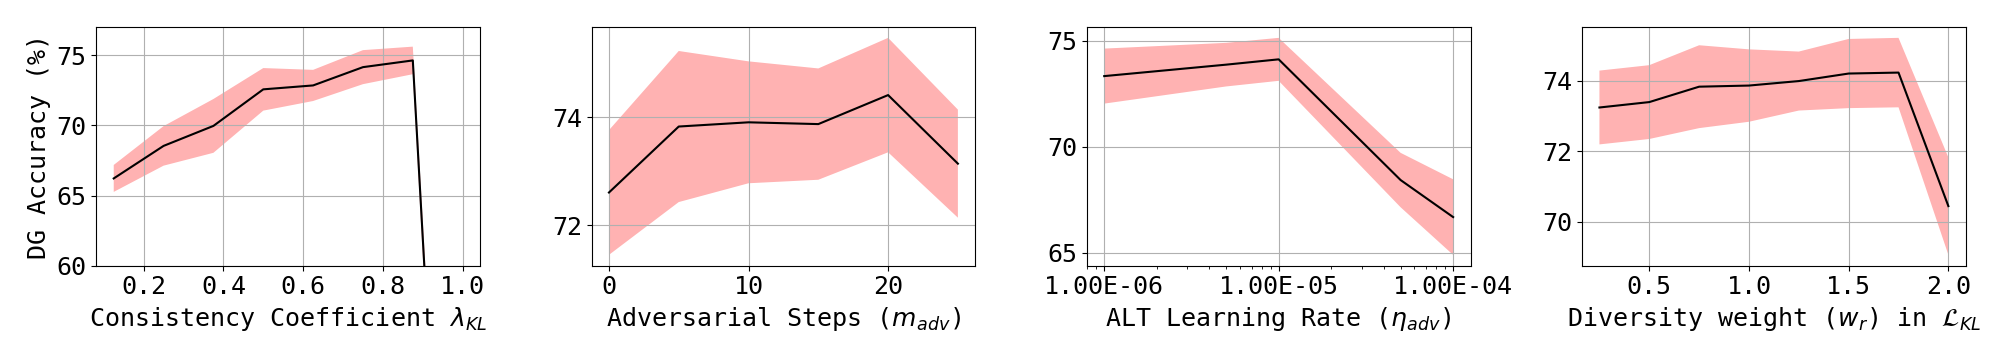
\includegraphics[width=\linewidth]{alt/figures/digits_hyperparam.png}
    \caption{\small{\textbf{Ablation Analysis:} We study the effect of each hyper-parameter in ALT on the average accuracy using the Digits benchmark. For each experiment we show 1 standard deviation around the mean over 5 runs. We observe that the consistency (left most) is generally important until a certain point, after which it becomes harmful; (left center) taking more adversarial steps improves performance; (right center) similarly, a small learning rate is preferred in training the adversary network, $g$, and performance degrades as the learning rate increases; (right most) Surprisingly, we find that the trade-off between diversity and ALT is non- trivial and dataset dependent.}}
    \label{fig:digits_hp}
\end{figure*}

\begin{table*}[t]
    \centering
    % \small
    \resizebox{\linewidth}{!}{
    \begin{tabular}{@{}l ccc ccc ccc ccc c@{}}
        \toprule
        \textbf{Method} & \textbf{A$\rightarrow$C} & \textbf{A$\rightarrow$S} & \textbf{A$\rightarrow$P} & \textbf{C$\rightarrow$A} & \textbf{C$\rightarrow$S} & \textbf{C$\rightarrow$P} & \textbf{S$\rightarrow$A} & \textbf{S$\rightarrow$C} & \textbf{S$\rightarrow$P} & \textbf{P$\rightarrow$A} & \textbf{P$\rightarrow$C} & \textbf{P$\rightarrow$S} & \textbf{Average}\\
        \midrule
        ERM                                 & 62.3 & 49.0 & 95.2 & 65.7 & 60.7 & 83.6 & 28.0 & 54.5 & 35.6 & 64.1 & 23.6 & 29.1 & 54.3\\
        JiGen~\citep{carlucci2019domain}     & 57.0 & 50.0 & 96.1 & 65.3 & 65.9 & 85.5 & 26.6 & 41.1 & 42.8 & 62.4 & 27.2 & 35.5 & 54.6\\
        ADA~\citep{volpi2018generalizing}    & 64.3 & 58.5 & 94.5 & 66.7 & 65.6 & 83.6 & 37.0 & 58.6 & 41.6 & 65.3 & 32.7 & 35.9 & 58.7 \\
        AugMix~\citep{hendrycks2019augmix}   & 68.4 & 54.6 & 95.2 & 74.3 & 66.7 & 87.3 & 40.0 & 57.4 & 46.8 & 67.3 & 26.8 & 41.4 & 59.6 \\
 
        RandConv~\citep{xu2020robust}        & 61.1 & 60.5 & 87.3 & 57.1 & 72.9 & 73.7 & 52.2 & 63.9 & 46.1 & 61.3 & 37.6 & 50.5 & 60.3\\
        SagNet~\citep{nam2021reducing}       & 67.1 & 56.8 & 95.7 & 72.1 & 69.2 & 85.7 & 41.1 & 62.9 & 46.2 & 69.8 & 35.1 & 40.7 & 61.9 \\
        \midrule 
        ALT$_{g-only}$                  & 63.5 & 63.8 &	94.9 & 68.9 & 74.4 & 84.6 & 39.7 & 61.1 & 49.3 &	68.8 & 43.4 & 50.8 & \textbf{63.6}\\
        ALT$_{RandConv}$                    & 63.6 & 65.8 & 92.5 & 69.1 & 75.1 & 84.5 & 40.1 & 61.7 & 50.8 & 68.4 & 43.4 & 55.2 & \textbf{64.2}\\
        ALT$_{AugMix}$                      & 65.7 & 68.2 & 93.2 & 71.9 & 74.2 & 86.0 & 40.2 & 62.9 & 49.1 & 68.5 & 43.5 & 53.3 & \textbf{64.7}\\
        % AugMax                            & 85.4 & 79.6 & 90.1 & 77.1 & 77.4 & 84.3 & 37.0 & 41.9 & 45.9 & 66.8 & 54.6 & 53.5 & 66.1 \\
        \bottomrule 
    \end{tabular}
    }
    \caption[SSDG PACS]{
        Single-source domain generalization accuracy (\%) on PACS~\citep{csurka2017domain}. 
        \textit{X$\rightarrow$Y} implies X is the source dataset and Y is the target dataset.
        \textit{P: photo; A: art-painting; C: cartoon; S: sketch.}
        Performance is reported as mean of 5 repetitions\footnotemark[1].
    }
    \label{tab:results_pacs}
\end{table*}


\subsection{PACS}
\footnotetext{$^*$standard deviation values are in the supplementary material.}
\paragraph{Baselines.}
Our baselines include JiGen~\citep{carlucci2019domain}, adversarial data augmentation (ADA)~\citep{volpi2018generalizing}, AugMix, RandConv, and SagNet~\citep{nam2021reducing} which is designed to reduce style bias using normalization techniques.
We use ResNet18~\citep{he2016deep} pre-trained on ImageNet as our model architecture and train all models for $2000$ iterations with batch-size of $32$, learning rate $0.004$, \texttt{SGD} optimizer with cosine annealing learning rate scheduler, weight decay of $0.0001$, and momentum $0.9$.
For ALT, we set consistency coefficient $\lambda_{KL}{=}0.75$, adversarial learning rate $\eta_{adv}{=}5e{-}5$, number of adversarial steps $m_{adv}{=}10$ and $w_r{=}1.0$.

\paragraph{Results.}
Results are shown in Table~\ref{tab:results_pacs}.
We observe that ALT without a diversity module (ALT$_{g-only}$) surpasses generalization performance of all prior methods including diversity methods RandConv and AugMix and the previous best SagNet~\citep{nam2021reducing}.
ALT with adaptive diversity further improves the results and ALT$_{AugMix}$ establishes a new state-of-the-art accuracy of $64.7\%$.
The most difficult target domains for previous methods has been \textit{Sketch (S)} since this is a set of rough human-drawn black-and-white sketches of real-life objects; the difficluty can be observed in terms of performance in columns $A{\rightarrow}S$, $C{\rightarrow}S$, and $P{\rightarrow}S$.
ALT significantly improves the performance on the sketch target domain, compared to the previous best.
ALT is also the best when generalizing from photos as the source to C,S,A as targets.
This is a very realistic setting since large-scale natural image datasets such as ImageNet~\citep{deng2009imagenet} are widely used and publicly available, while datasets for sketches, cartoons, and painting are not.

\begin{table*}[t]
    \centering
    % \small
    \resizebox{\linewidth}{!}{
    \begin{tabular}{@{}l ccc ccc ccc ccc c@{}}
        \toprule
        \textbf{Method} & \textbf{A$\rightarrow$C} & \textbf{A$\rightarrow$P} & \textbf{A$\rightarrow$R} & \textbf{C$\rightarrow$A} & \textbf{C$\rightarrow$P} & \textbf{C$\rightarrow$R} & \textbf{P$\rightarrow$A} & \textbf{P$\rightarrow$C} & \textbf{P$\rightarrow$R} & \textbf{R$\rightarrow$A} & \textbf{R$\rightarrow$C} & \textbf{R$\rightarrow$P} & \textbf{Average}\\
        \midrule
        ERM                                 & 42.61 & 59.18 & 69.45 & 48.37 & 56.09 & 59.38 & 46.07 & 40.18 & 68.19 & 63.12 & 45.13 & 74.34 & 56.00 \\
        AugMix~\citep{hendrycks2019augmix}   & 45.31 & 61.88 & 71.88 & 49.30 & 58.93 & 62.24 & 50.04 & 42.59 & 71.51 & 64.10 & 47.56 & 75.95 & 58.44 \\
        RandConv~\citep{xu2020robust}    & 43.98 & 55.28 & 67.31 & 45.49 & 56.58 & 59.03 & 43.80 & 43.19 & 66.50 & 57.62 & 48.26 & 72.97 & 55.00\\
        SagNet~\citep{nam2021reducing}   & 42.18 & 56.03 & 67.34 & 46.68 & 53.89 & 57.88 & 45.49 & 40.09 & 67.11 & 61.39 & 48.32 & 72.79 & 54.93\\
        \midrule 
        ALT$_{g-only}$                  & 47.26 & 61.14 & 71.21 & 48.88	& 57.81 & 60.99	& 48.15 & 46.70 & 69.30 & 64.85 & 52.84 & 76.28 & \textbf{58.78} \\
        ALT$_{RandConv}$                & 48.33 & 61.19 & 71.75 & 50.13 & 58.82 & 62.26 & 49.21 & 47.03 & 70.53 & 64.88 & 53.10 & 76.07 & \textbf{59.44}\\
        ALT$_{AugMix}$                  & 48.06 & 61.16 & 71.12 & 50.43 & 58.84 & 61.84 & 49.32 & 47.55 & 70.64 & 64.86 & 53.27 & 76.29 & \textbf{59.45} \\
        \bottomrule 
    \end{tabular}
    }
    \caption[SSDG Office-Home]{Single-source domain generalization accuracy (\%) on Office-Home~\citep{venkateswara2017deep} 
    % with mean and standard deviation 
    over five repetitions. 
    \textit{X$\rightarrow$Y} implies X is the source dataset and Y is the target dataset.
    \textit{R: real; A: art; C: clipart; P: product.}
    Performance is reported as mean of 5 repetitions\footnotemark[1].
    % ; detailed results with standard deviation values are in the supplementary material.
    }
    \label{tab:results_officehome}
\end{table*}
\subsection{Office-Home}
\paragraph{Baselines.}
For PACS, we follow the protocol from the previous state-of-the-art Sagnet~\citep{nam2021reducing} and use ResNet50 as the model architecture.
% and identical training settings and hyperparameters as PACS.
Note that we do not perform any hyperparameter tuning for OfficeHome and directly apply identical training settings and hyperparameters from PACS.

\paragraph{Results.}
Table~\ref{tab:results_officehome} shows the results on Office-Home.
We observe that RandConv (previous best on Digits) and SagNet (previous best on PACS) perform worse than ERM on OfficeHome, while AugMix is better by $2.44\%$.
All three variants of ALT surpass prior results, with ALT$_{AugMix}$ resulting in the best accuracy of $59.45\%$.
The most difficult target domain for previous methods are \textit{Art (A)} and \textit{Clipart (C)}, possibly because both sets have images with white backgrounds, while real world photos (R) and product images are naturally occurring.
ALT improves performance in each case when with A or C as target domain.
An observation similar to PACS can also be made here -- ALT is the best model under the realistic setting of generalizing from widely available real photos (R) to other domains.

\section{Analysis of ALT}
In this section we study the various components of ALT, and provide insights into their impact on generalization. 
\begin{figure*}
    \centering
    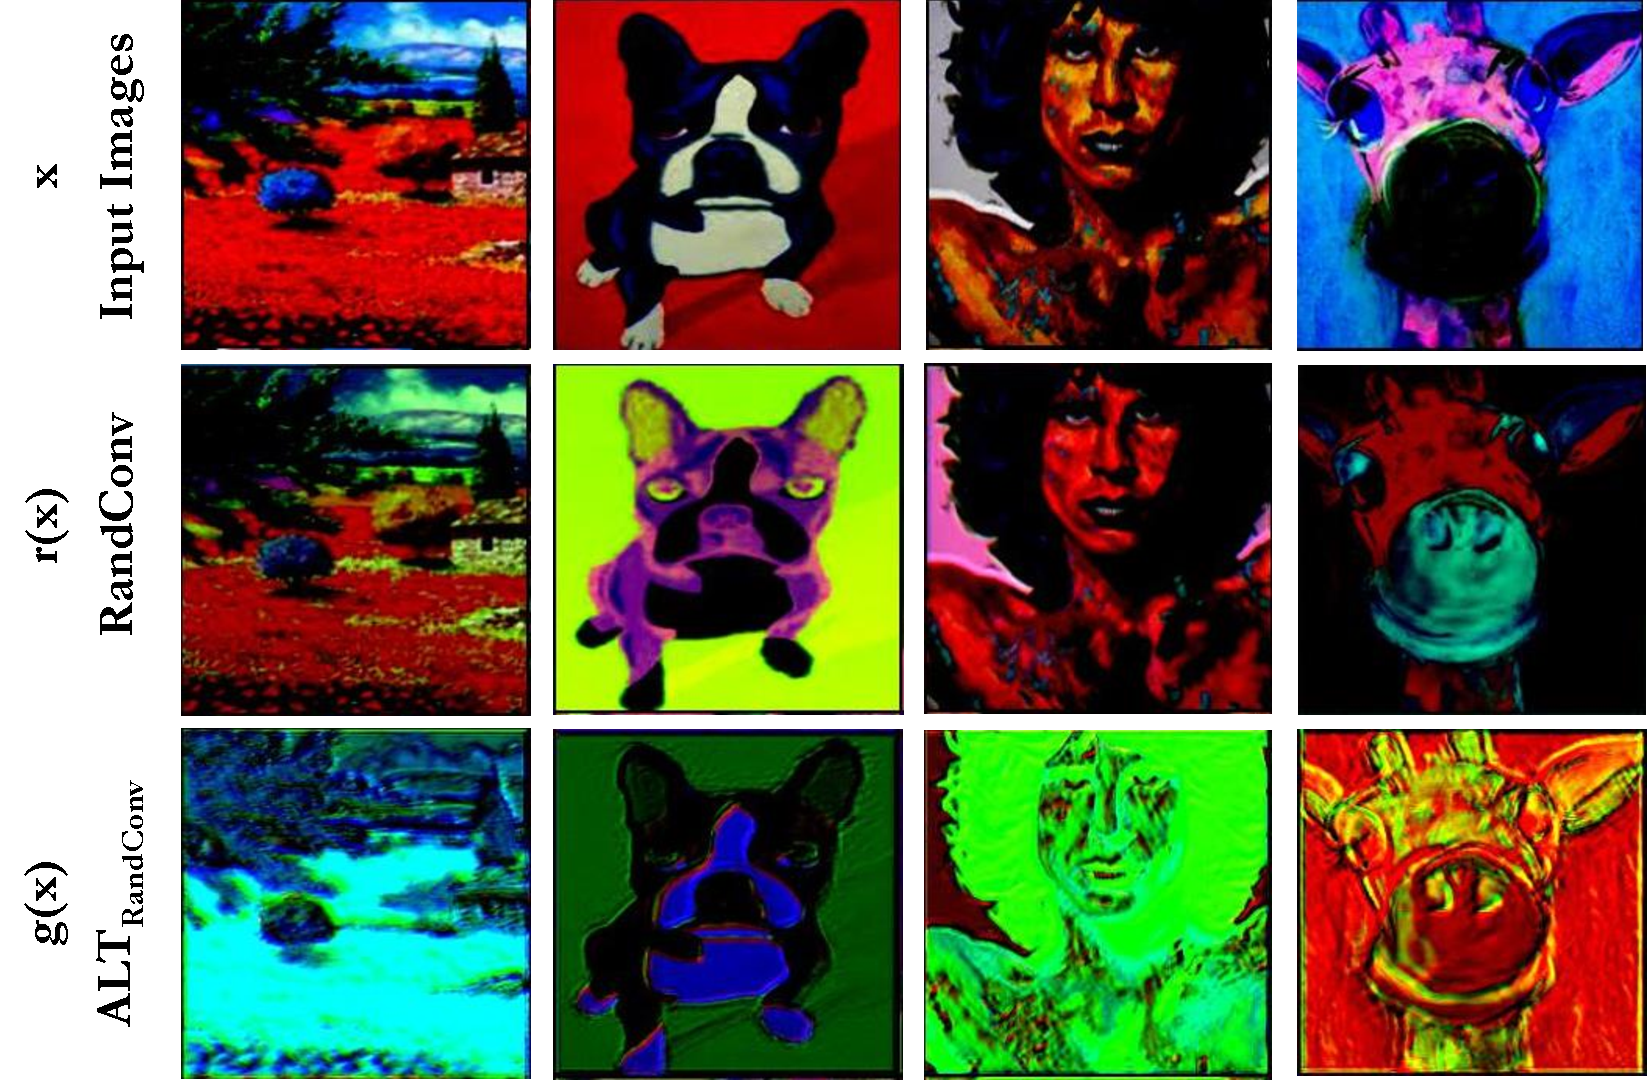
\includegraphics[width=0.48\linewidth]{alt/figures/viz_randconv_alt.pdf}
    \quad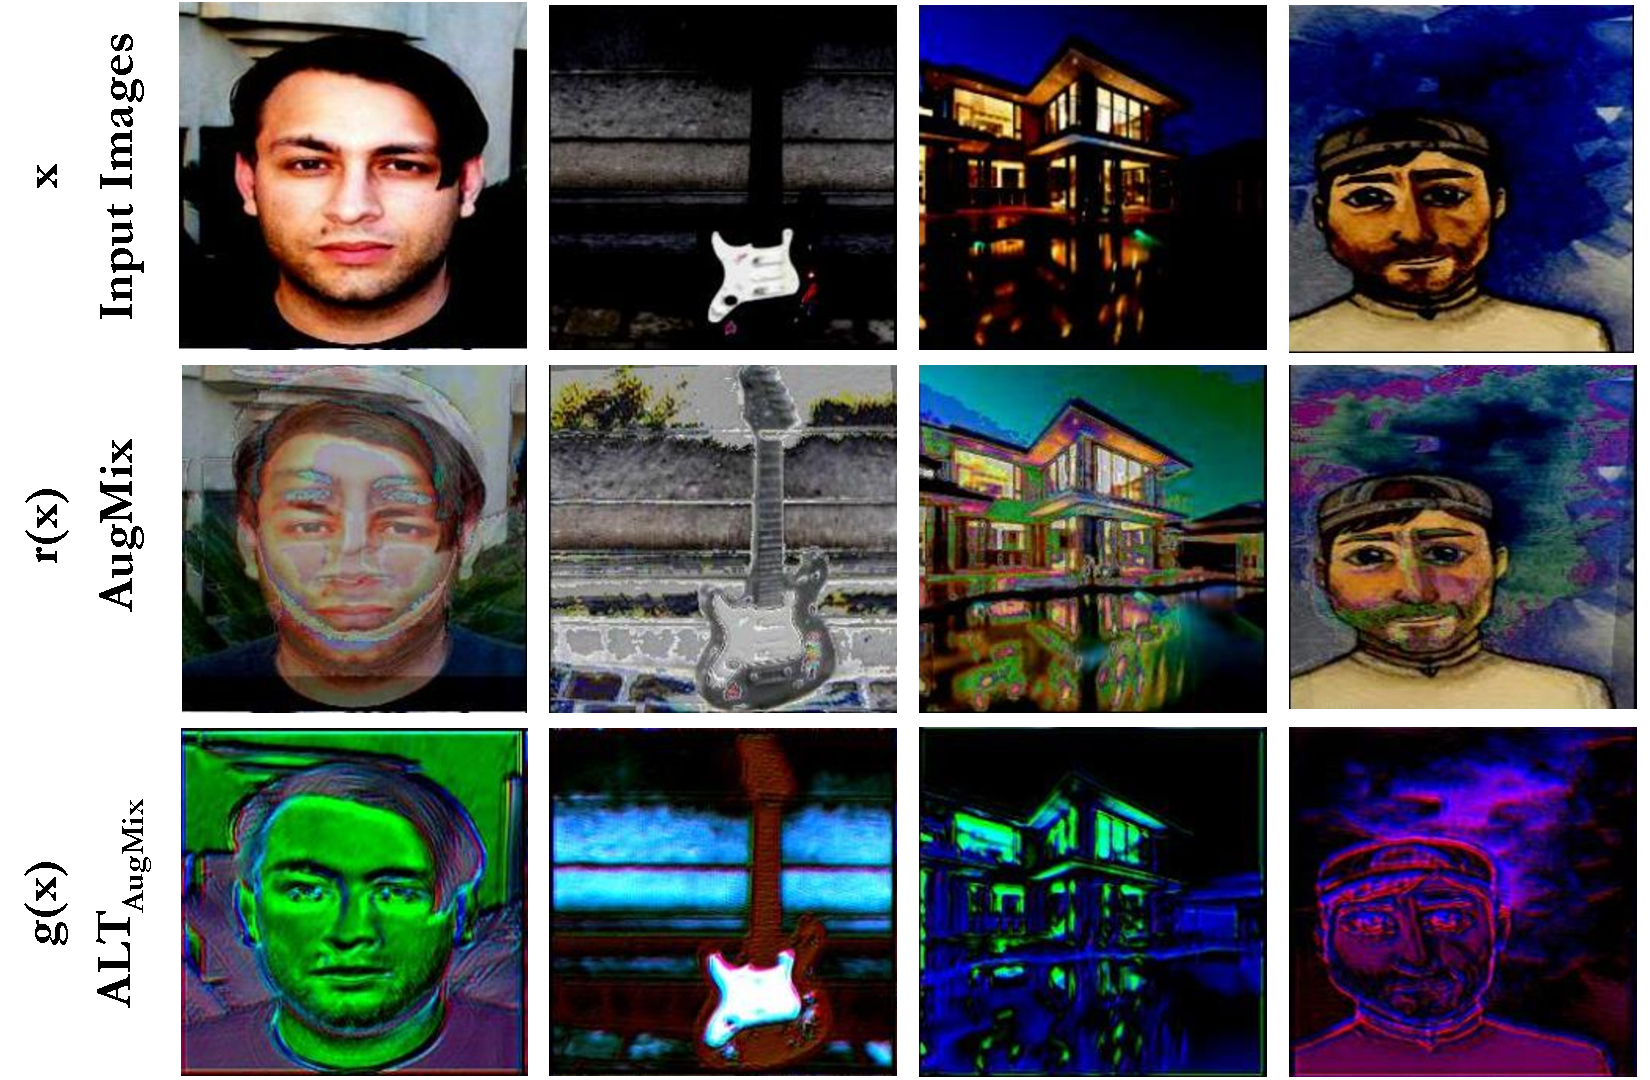
\includegraphics[width=0.48\linewidth]{alt/figures/viz_augmix_alt.pdf}
    \caption{Comparison of images transformed by data augmentation techniques RandConv \textit{(left)} and AugMix \textit{(right)} and their combination with ALT (ALT$_{RandConv}$ and ALT$_{AugMix}$), 
    illustrating the wide range of transformations learned by ALT.}
    \label{fig:viz_augs}
\end{figure*}

\paragraph{ALT is better than na\"ive diversity} Our first big insight is that ALT without an explicit diversity module still outperforms all the top performing methods across the benchmarks we evaluated on, indicating that learned adversarial transformations are a powerful way to train classifiers for generalization. They include diversity (achieved through random initializations) and adversarial images that help expose the classifier to large distribution shifts. Our next observation is that ALT makes the choice of diversity module fairly arbitrary. We see this effect on multiple benchmarks -- for example, on the Digits benchmark shown in  \Cref{tab:results_digits}, AugMix has a relatively poor generalization performance when compared with the baseline ERM whereas ALT$_{Augmix}$ achieves state of the art. This is again seen in the Office-Home benchmark shown in \Cref{tab:results_officehome}, where RandConv is worse than ERM, but ALT$_{RandConv}$ is the best performing method. We show examples of the image transformations learned with ALT in Figure~\ref{fig:viz_augs}, and it is clear that ALT achieves far more diverse and larger transformations of the input images than either AugMix or RandConv.

% - basically talk about diversity alone (Augmix/RC) -- see some boost, but varying results on each benchmark.
% MNIST -- augmix boosts by 1\% barely, but big jump for RandConv.
% On PACS and OfficeHome, AugMix is better than RandConv.
% - ALT without diversity is better than Diversity alone
% - ALT can better adapt its diversity when combined with RandConv and Augmix -- the combination and interplay between the adversarial cost and consistency, is key.


\paragraph{ALT Hyperparameters.}
The four main hyper-parameters that control ALT are: the consistency coefficient $\lambda_{KL}$ in Equation~\ref{alt:eq:L_KL} which decides the proportion between the classifier loss and KL-divergence consistency between transformations, 
number of adversarial steps and learning rate in the adversarial maximization of Equation~\ref{alt:eq:adv_max}, and the diversity weight $w_r$ which controls the interaction between the diversity module $r()$ and the adversary network $g()$ in Equation~\ref{alt:eq:p_mix}.
We investigate the effect of each of these on domain generalization accuracy in Figure~\ref{fig:digits_hp}.
The first plot shows that the consistency coefficient $\lambda_{KL}$ is impactful and a higher value leads to better generalization.
However at $\lambda_{KL}=1.0$ the accuracy degenerates to random performance; this is expected as the classifier loss gets $1-\lambda_{KL}{=}0$ weight.
From the second and third plots, we observe that an optimal value exists around 20 adversarial steps and learning rate of $1e{-}5$.
There is a fast drop in generalization at higher learning rates.
Increasing the diversity weight also leads to increase in generalization, however at $w_r{=}2$ the performance drops and corresponds to "diversity only" settings.
Clearly, the adversarial component is a critical factor that causes improvements in generalization.

\begin{table}[t]
    \centering
    % \small
    \begin{tabular}{@{}lccc@{}}
        \toprule
        \textbf{Architecture} & \textbf{Digits Average} & \textbf{PACS Average} \\
        \midrule
        FCN (2 layers) & 72.75 & 63.40 \\
        FCN (3 layers) & 73.74 & 63.92\\
        FCN (4 layers) & 74.10 & 64.41 \\
        FCN (5 layers) & 73.87 & 64.20 \\
        FCN (6 layers) & 74.15 & 63.78\\
        % ResNetGen-6~\cite{johnson2016perceptual} & \\
        % UNet-10~\cite{ronneberger2015u} & \\
        \bottomrule
    \end{tabular}
    \caption{Effect of the architecture of the adversity network $g$ on average domain generalization on the PACS and Digits benchmarks.}
    \label{tab:gvars}
\end{table}

% \begin{table}[t]
%     \centering
%     \begin{tabular}{cc}
%         \toprule
%         \textbf{Method}     & \textbf{DG Avg.}\\
%         \midrule
%         RandConv            & \\
%         AugMix              & 59.56\\
%         ALT$_{RandConv}$    & \\
%         ALT$_{AugMix}$      & \\
%         ALT$_{none}$        & \\
%         \bottomrule
%     \end{tabular}
%     \caption{PACS DG Average}
%     \label{tab:ablation_hd}
% \end{table}

\paragraph{Complexity of Adversary Network.}
In our experiments on the benchmark datasets we have used a simple fully convolutional network (FCN) with 5 convolutional layers.
We conduct additional analysis to understand how this choice affects generalization performance, and compare performance when using between 2 and 6 convolutional layers.
% We compare FCN with number of layers between 2 and 6.
% and two additional architectures -- U-Net-10~\citep{ronneberger2015u} with 5 downsampling and 5 upsampling operations (UNet-10) and a ResNet based generator (ResNetGen-6) with 3 downsampling and 3 upsampling operations. operations~\citep{johnson2016perceptual}.
% Note that the UNet and ResNet generators are considerably more sophisticated than FCN, and contain bottleneck architectures and skip connections.
We reuse all other training settings from our benchmark model $ALT_{RandConv}$ on both Digits and PACS.
For PACS, we observe that all ALT models compared are better than previous baselines including AugMix and RandConv.
For Digits, we observe that performance of ALT with a 2-layer $g$ is close to RandConv, and is greater than all previous baselines for higher depth of the network.
Increasing the number of layers, i.e., increasing the complexity of the adversary network leads to better performance upto 5 layers, even with the same learning rate.

% \paragraph{Qualitative Comparison of Diverse Augmentations}

% \begin{figure}[t]
%     \centering
%     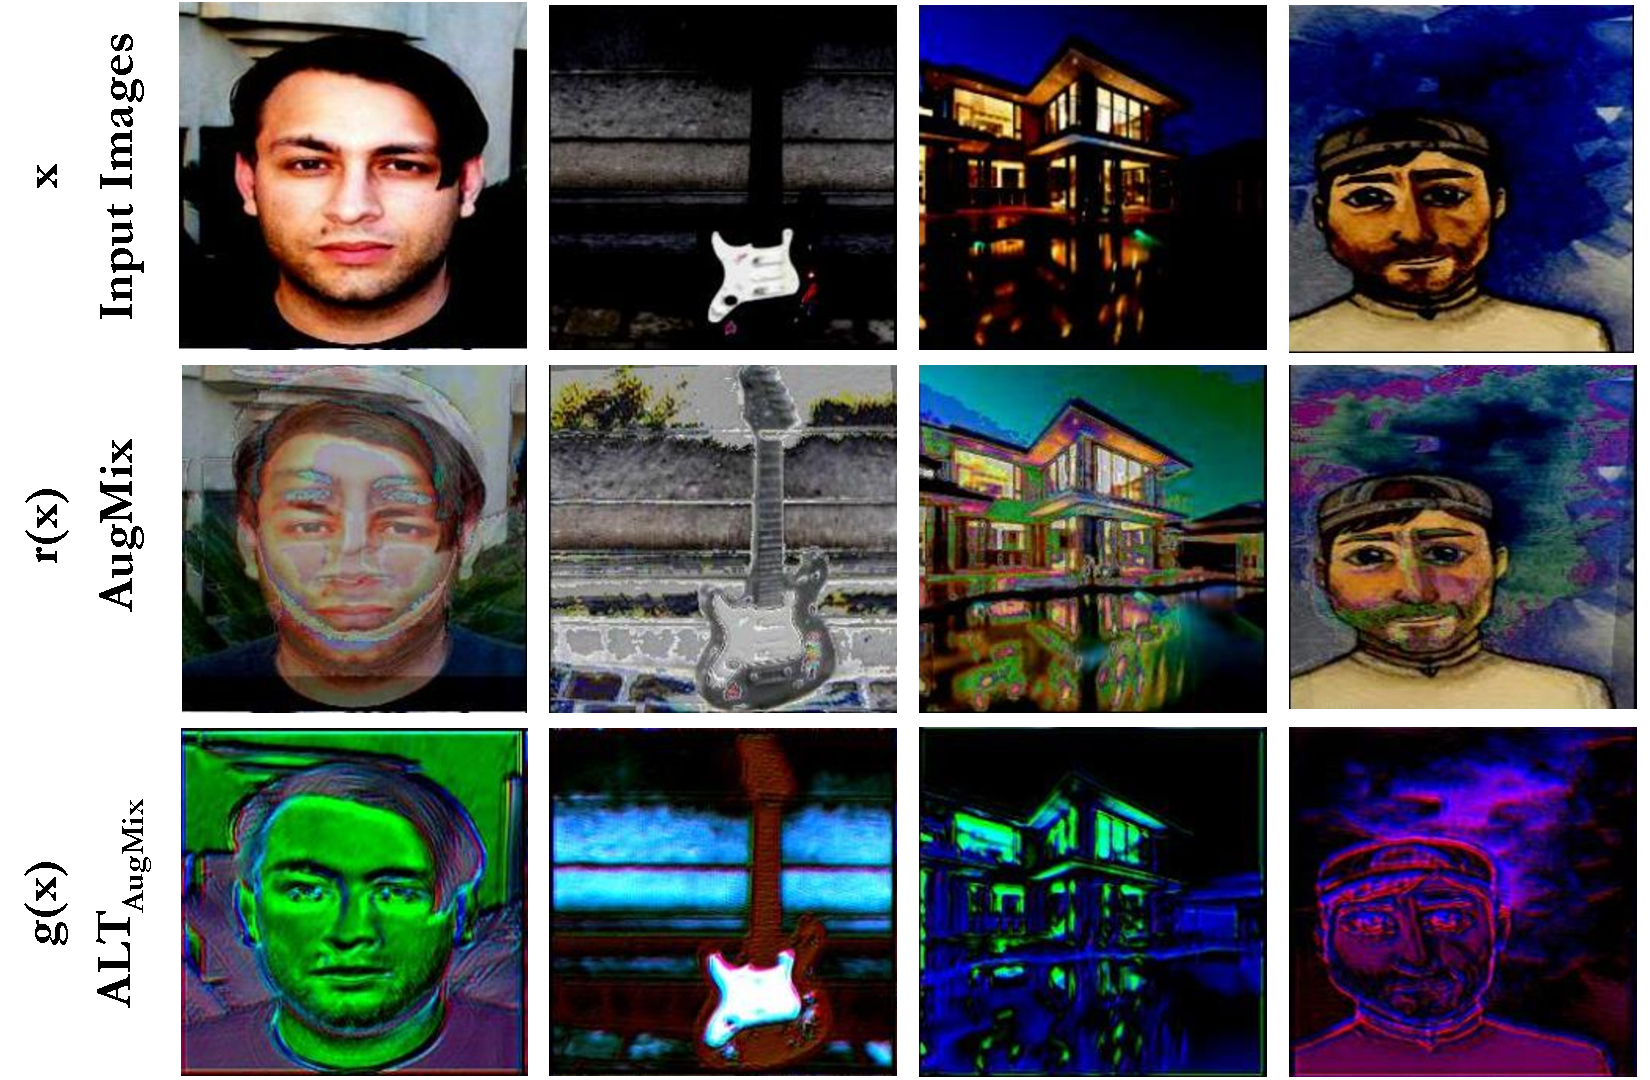
\includegraphics[width=\linewidth]{alt/figures/viz_augmix_alt.pdf}
%     \caption{Comparison of transformed images for AugMix and ALT$_{AugMix}$.}
%     \label{fig:viz_augmix}
% \end{figure}
% In Figure~\ref{fig:viz_augs} we illustrate the difference between the augmentations generated by RandConv, AugMix, ALT$_{g-only}$, ALT$_{RandConv}$ and ALT$_{AugMix}$.


\section{Conclusion}
In this paper, we address the problem of single source domain generalization. Our approach, Adversarially Learned Transformations (ALT) uses a randomly initialized convolutional network to learn plausible image transformations of the source domain that can fool the classifier. These images are used to enforce a consistency with the predictions on clean images. We showed that this strategy outperforms all existing techniques on multiple benchmarks because it is able to generate a diverse set of large transformations of the source domain. 
%
% In this paper, we started with the hypothesis that diversity alone or adversarial training alone is not enough for generalizing to unseen domains in the single-source domain generalization setting, as was confirmed by our experiments and mixed results on prior methods on different benchmarks.
We also find that ALT can be naturally combined with existing diversity modules like RandConv or AugMix to improve their performance (sometimes significantly). We also studied the different parts of ALT through extensive ablations and analysis to obtain insights into its performance gains. Our studies indicate that na\"ive diversity alone is insufficient, but needs to be combined adversarial transformations to maximize generalization performance. 


